\documentclass[a4paper,11pt]{article}
\usepackage[utf8]{inputenc}
\usepackage{tikz}
\usepackage{xparse}
\usetikzlibrary{positioning,fit,calc}

\thispagestyle{empty} % no pagenumber. The form should be a stand alone macro... later.

\definecolor{SEPAOrange}{RGB}{254,213,161}
\definecolor{SEPADOrange}{RGB}{253,185,19}
\definecolor{SEPABlindcolor}{RGB}{255,0,0}



% switch on expl3 syntax
% (_ and : become part of macro names; spaces are ignored; ~ is normal space)
\ExplSyntaxOn
% make @ available as part of macro name
\makeatletter


%\formlines{\xs}{\yh}{5}{22}{IBAN}

\NewDocumentCommand { \formlines }{mmmmm}
%\formlines{x,y, width, label}
{

\filldraw[color=white] (#1, #2) rectangle (#4 * #3 + #1, #2 +1.5 * 4.2333 - 1.5); %Recepient 27 Char

% draw label
\node[every~form~label, anchor=south~west,align=left] at (#1,#2) {#5};

\foreach \x in {2,...,#4}
{
 \draw[color=SEPAOrange, line~width=0.3mm] (#1 + \x * #3 -#3, #2 ) -- (#1 + \x * #3 -#3, #2 + 1.5 * 4.2333 - 1.5);
 \draw[color=SEPAOrange, line~width=0.8mm] (#1 + \x * #3 -#3, #2 + 3  ) -- (#1 + \x * #3 -#3, #2 + 1.5 * 4.2333 - 1.5);
}

}



% switch off expl3 syntax and @
\ExplSyntaxOff\makeatother

\tikzset{
    every form field/.style = {
        fill=white,
        inner sep=0pt,
        minimum height=4mm,
        align=center,
    },
    every form field middle/.style = {
        every form field,
        form field middle,
    },
    every form field start/.style = {
        every form field,
        form field start,
        anchor=south west,
    },
    every form field end/.style = {
        every form field,
        form field end,
    },
    every form label/.style = {
        fill=white, text=SEPABlindcolor,
        inner sep=1pt,
        outer sep=0pt,
        font=\tiny\sffamily\bfseries,
    },
    every form digit/.style = {
        anchor=base,
        font=\ttfamily,
        inner sep=0pt,
    },
    every form divider/.style = {
        fill=black,
        inner sep=0pt,
        outer sep=0pt,
        anchor=south,
        minimum width=\formdividerwidth,
        minimum height=\formdividerheight,
    },
}



\begin{document}


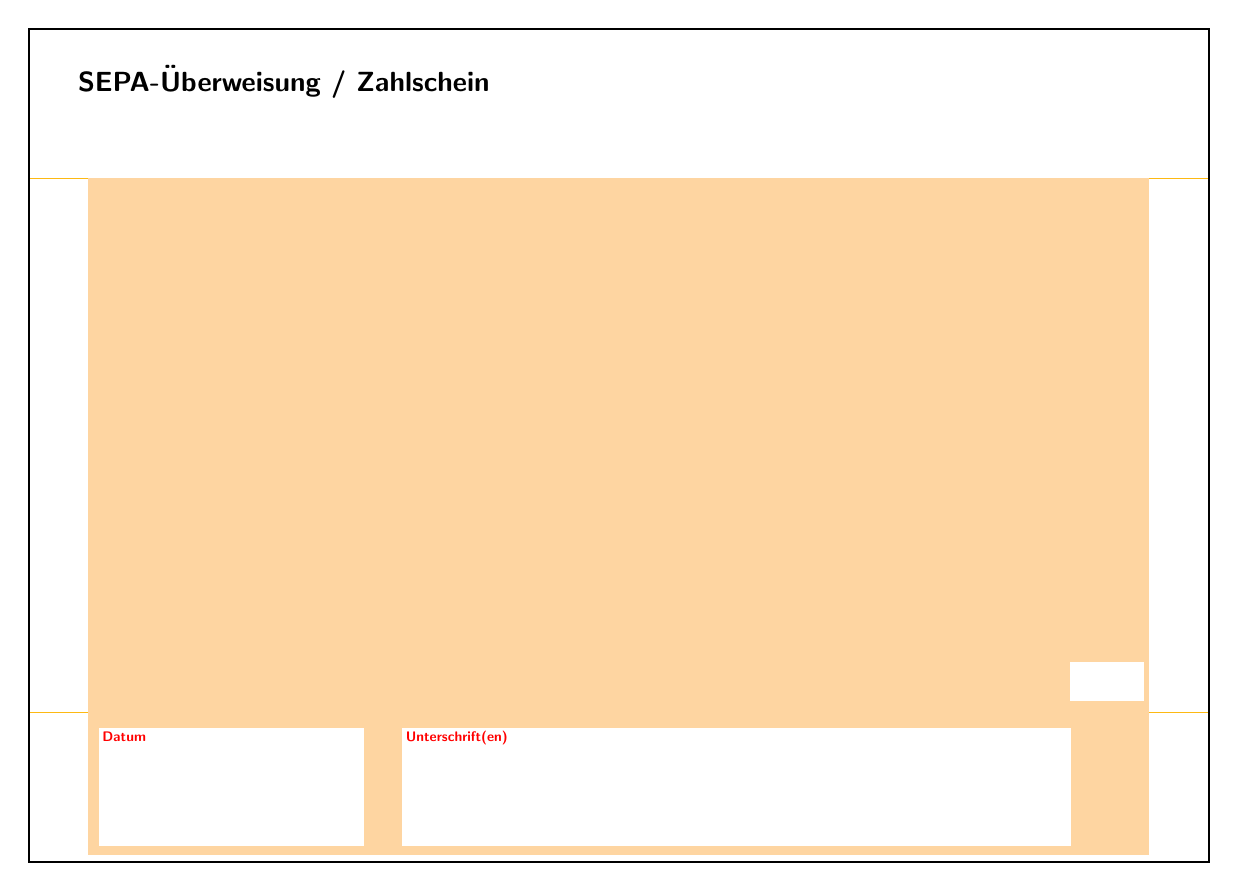
\begin{tikzpicture}[x=1 mm, y=-1 mm, node distance=4 pt]

\pgfmathsetmacro{\yh}{4.2333} % y heigth step defined as 1/6 inch =>  1/6 * 25.4 mm = 4.2333 mm
\pgfmathsetmacro{\xs}{9} % x start (own definition)
\pgfmathsetmacro{\xe}{141.5} % x end (own definition)
\pgfmathsetmacro{\widefield}{4.9859} % def: 134.62 mm / 27
\pgfmathsetmacro{\narrowfield}{3.9594} % def: 134.62 mm/ 34

\draw[color=SEPADOrange] (0, 4.5 *\yh) --(149.86, 4.5*\yh); upper dark orange line
\draw[color=SEPADOrange] (0, 20.5 *\yh) --(149.86, 20.5*\yh); lower dark orange line
\filldraw[draw=black,color=SEPAOrange] (7.62, 4.5*\yh) rectangle (149.86-7.62,105.83-1); %orange background

\node[anchor=north west,align=left,font=\sffamily] at (5, 0.8*\yh) {\bfseries{SEPA-Überweisung} / Zahlschein};


%\filldraw[draw=black,color=white] (\xs, 5*\yh) rectangle (\xe, 6.5*\yh -1.5); %Recepient 27 Char
\formlines{\xs}{5 * \yh}{\widefield}{27}{Zahlungsempfänger}


%\filldraw[draw=black,color=white] (\xs, 7*\yh) rectangle (\xe, 8.5*\yh -1.5); %IBAN 34 Char
\formlines{\xs}{7 * \yh}{\narrowfield}{34}{IBAN}


%\filldraw[draw=black,color=white] (\xs, 9*\yh) rectangle (\xe, 10.5*\yh -1.5); %BIC
\formlines{\xs}{9 * \yh}{\widefield}{9}{BIC}


%\filldraw[draw=black,color=white] (\xe-12*5, 11*\yh) rectangle (\xe, 12.5*\yh -1.5); %Value 12 Char 
\formlines{\xe - 12*5}{11 * \yh}{\widefield}{12}{Betrag: Euro, Cent}


%\filldraw[draw=black,color=white] (\xs, 13*\yh) rectangle (\xe, 14.5*\yh -1.5); %Subject1
\formlines{\xs}{13 * \yh}{\widefield}{27}{Kunden-Referenznummer - Verwendungszweck, ggf. Name und Anschrift des Zahlers}
\formlines{\xs}{15 * \yh}{\widefield}{27}{noch Verwendungszweck}
\formlines{\xs}{17 * \yh}{\widefield}{27}{Angaben zum Kontoinhaber/Zahler: Name, Vorname/Firma, Ort}


%\filldraw[draw=black,color=white] (\xs, 19*\yh) rectangle (\xs+22*5, 20.5*\yh -1.5); % IBAN 22 Char
\formlines{\xs}{19 * \yh}{\widefield}{22}{IBAN}

\filldraw[draw=black,color=white] (149.86-17.59, 19* \yh) rectangle (\xe, 20.5*\yh -1.5); % counter
\filldraw[draw=black,color=white] (\xs, 21* \yh) rectangle (42.52, 24.5*\yh); % date
\node[every form label, anchor=north west,align=left] at (\xs, 21* \yh) {Datum};


\filldraw[draw=black,color=white] (42.52+5, 21*\yh) rectangle (149.86-17.59, 24.5*\yh); % signature
\node[every form label, anchor=north west,align=left] at (42.52+5, 21*\yh) {Unterschrift(en)};



\draw[draw=black,color=black, line width=0.3mm] (0,0) rectangle (149.86,105.83); % black border
%\draw[align=left] at (\yh,\yh) {SEPA-Überweisung};

%\filldraw[draw=black,color=SEPAOrange] (7.62, 4.5*\yh) rectangle (149.86-7.62,105.83-1); %orange background
%\formline*(\xs,7*\yh)[4mm]{22}{IBAN}[DE00 2105 0170 0012 3456 78]

%\formliner*(0,0)[4mm]{22}{IBAN}[DE00 2105 0170 0012 3456 78]
%\draw[color=red] (\xs, \yh) --(\xs+22*4mm, \yh); lower dark orange line % TESTRULER

\end{tikzpicture}
\end{document} 